\documentclass[usenames,dvipsnames,10pt,pdf,utf8,russian,aspectratio=43]{beamer}
\usepackage[english,russian]{babel}
\usepackage{cmap}
\usepackage[T2A]{fontenc}
\usepackage{subfig}
\usepackage{color}
\usepackage{tikz}
%\usepackage{tikz,fullpage}
\DeclareMathOperator*{\argmax}{arg\,max}
\DeclareMathOperator*{\argmin}{arg\,min}

\usetikzlibrary{arrows,automata}
\usetikzlibrary{positioning}

%
% Choose how your presentation looks.
%
% For more themes, color themes and font themes, see:
% http://deic.uab.es/~iblanes/beamer_gallery/index_by_theme.html
%


\mode<presentation>
{


  \usetheme{Boadilla}      % or try Darmstadt, Madrid, Warsaw, ...
  \usecolortheme{seagull} % or try albatross, beaver, crane, ..

 \usefonttheme{structurebold}  % or try serif, structurebold, ...
  \setbeamertemplate{navigation symbols}{}
  \setbeamertemplate{caption}[numbered]
} 


\captionsetup[subfloat]{labelformat=empty}
\title[Выбор модели]{Выбор модели глубокого обучения}
\author{Бахтеев Олег}
\institute{МФТИ}
\date{16.10.2019}

\begin{document}

\begin{frame}
  \titlepage
\end{frame}


\section{Сложность модели}
\begin{frame}{Сложность модели: зачем?}
\begin{figure}
  \centering
  \subfloat[Устойчивость моделей при возмущении выборки]{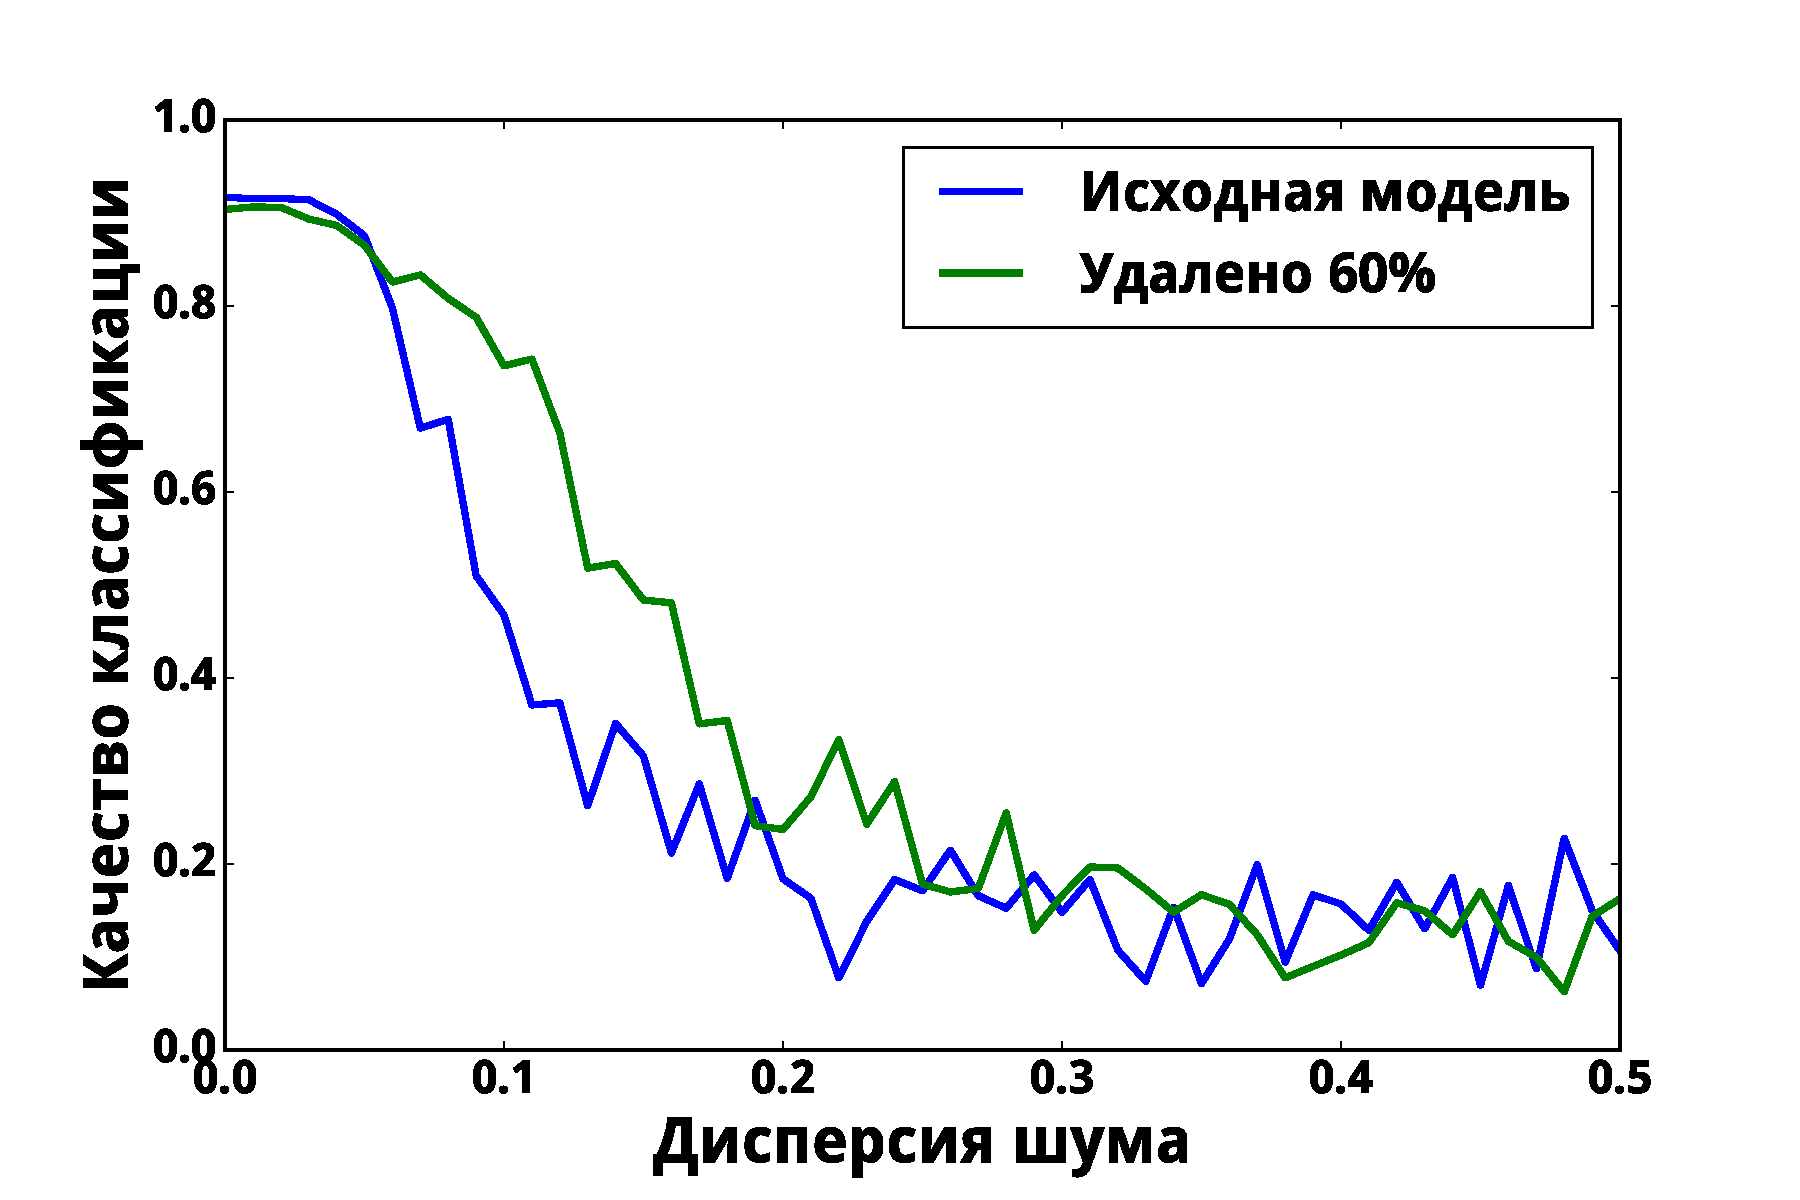
\includegraphics[width=0.4\textwidth]{noise.pdf}} 
 \subfloat[Качество классификации при удалении параметров]{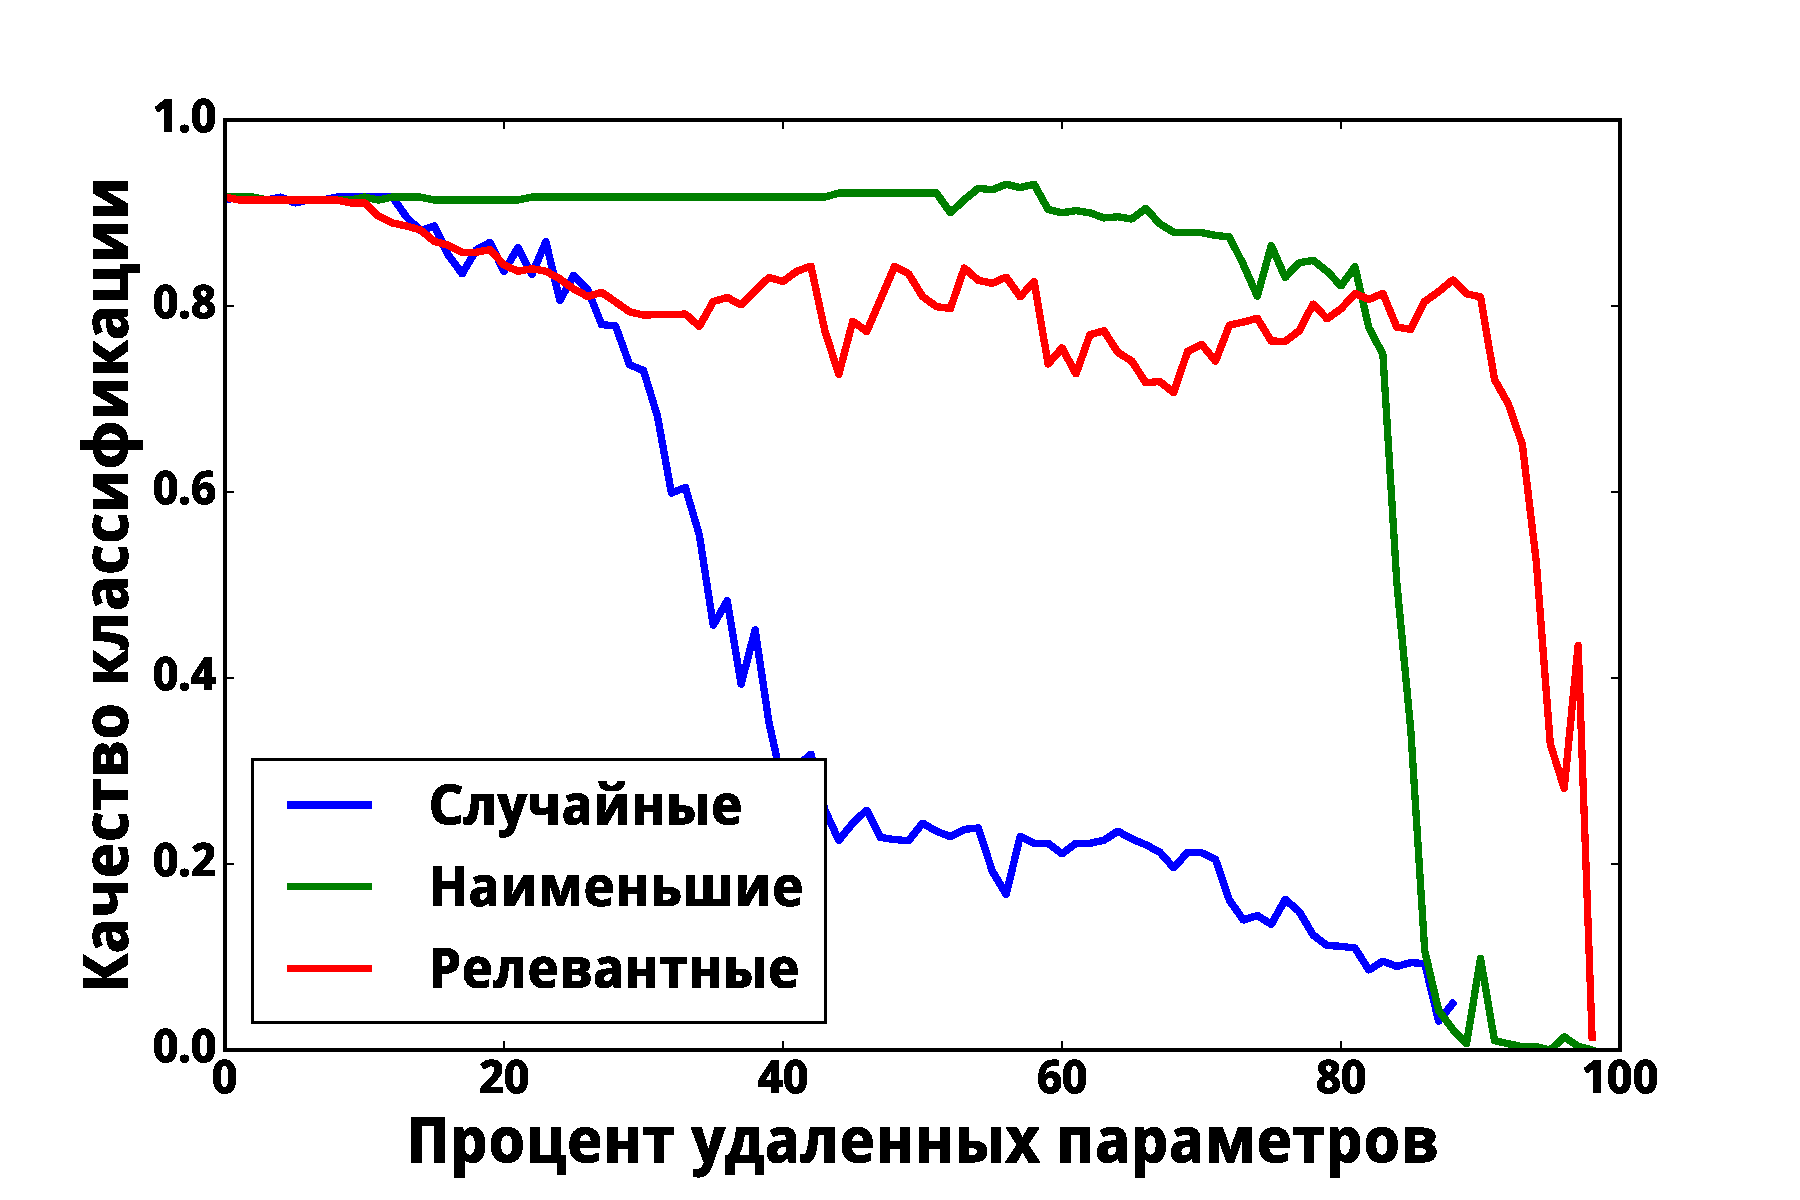
\includegraphics[width=0.4\textwidth]{pruning.pdf}}
\label{fig:1}\qquad

\end{figure}


\end{frame}

\begin{frame}{Сложность модели: зачем?}

\begin{figure}
  \centering
 {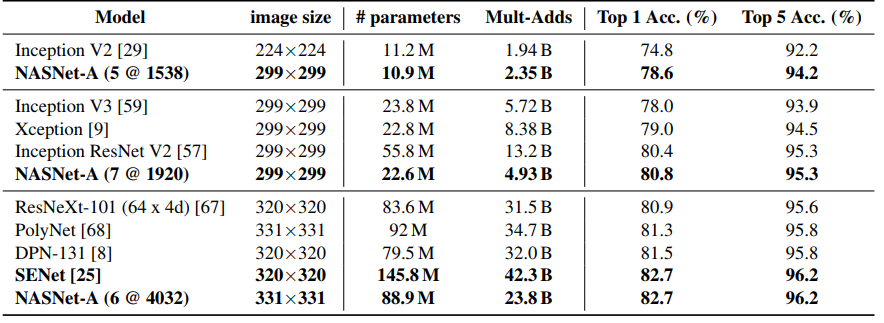
\includegraphics[width=\textwidth]{zoph.png}}
\label{fig:1}\qquad
\caption*{Zoph et al., 2017.  Сложность моделей отличается почти в два раза при одинаковом качестве.}
\end{figure}
\end{frame}

\begin{frame}{Глубокого обучение}
\begin{block}{Определение}
\textit{Моделью} $\mathbf{f}(\mathbf{w}, \mathbf{x})$ назовем дифференцируемую по параметрам $\mathbf{w}$ функцию из множества признаковых описаний объекта во множество меток:
\[
    \mathbf{f}: \mathbb{X} \times \mathbb{W} \to \mathbb{Y},
\] 
где $\mathbb{W}$ --- пространство параметров функции $\mathbf{f}$.
\end{block}
~\\~\\
\textbf{Особенность задачи}  выбора модели \textit{глубокого обучения} --- значительное число параметро в моделях приводит к неприменимости классических методов оптимизации и выбора модели. \\~\\

\textbf{Сложность модели:}
\begin{enumerate}
\item количество параметров;
\item количество суперпозиций внутри модели.
\end{enumerate}
\end{frame}


\begin{frame}{Принцип минимальной длины описания}
\[
\text{MDL}(\mathbf{f}, \mathfrak{D}) = L(\mathbf{f}) + L(\mathfrak{D}|\mathbf{f}),
\]
где $\mathbf{f}$ --- модель, $\mathfrak{D}$ --- выборка, $L$ --- длина описания в битах.
\\
\[
\text{MDL}(\mathbf{f}, \mathfrak{D}) \sim L(\mathbf{f}) + \textcolor{blue}{L(\mathbf{w}^*| \mathbf{f})} + \textcolor{red}{L(\mathfrak{D}|\mathbf{w}^*, \mathbf{f})},
\]
$\mathbf{w}^*$ --- оптимальные параметры модели.\\

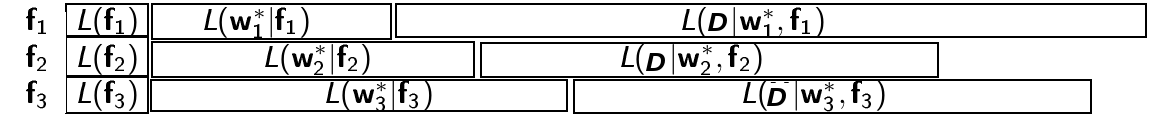
\includegraphics[width=\textwidth]{./mdl.png}

\end{frame}

\begin{frame}{MDL и Колмогоровская сложность}
\textbf{Колмогоровская сложность} --- длина минимального кода для выборки на предварительно заданном языке.

\textbf{Теорема инвариантности}\\
Для двух сводимых по Тьюрингу языков колмогоровская сложность  отличается не более чем на константу, не зависяющую от мощности выборки.\\

\textbf{Отличия от MDL}:
\begin{itemize}
\item Колмогоровская сложность невычислима.
\item Длина кода может зависеть от выбранного языка. Для небольших выборок теорема инвариантности не дает адекватных результатов.
\end{itemize}
\end{frame}


\begin{frame}{Связанный байесовский вывод}
\textit{Первый уровень:} выбираем оптимальные параметры:
\[
    \mathbf{w} = \argmax \frac{p(\mathfrak{D}|\mathbf{w})p(\mathbf{w}|\mathbf{h})}{p(\mathfrak{D}|\mathbf{h})},
\]

\textit{Второй уровень:} выбираем модель, доставляющую максимум обоснованности модели.

Обоснованность модели (``Evidence''):
\[
	p(\mathfrak{D}|\mathbf{h}) = \int_\mathbf{w} \textcolor{blue}{p(\mathfrak{D}|\mathbf{w})}\textcolor{red}{p(\mathbf{w}|\mathbf{h})} d\mathbf{w}.
\]


\begin{figure}
  \centering
  \subfloat[Схема выбора модели]{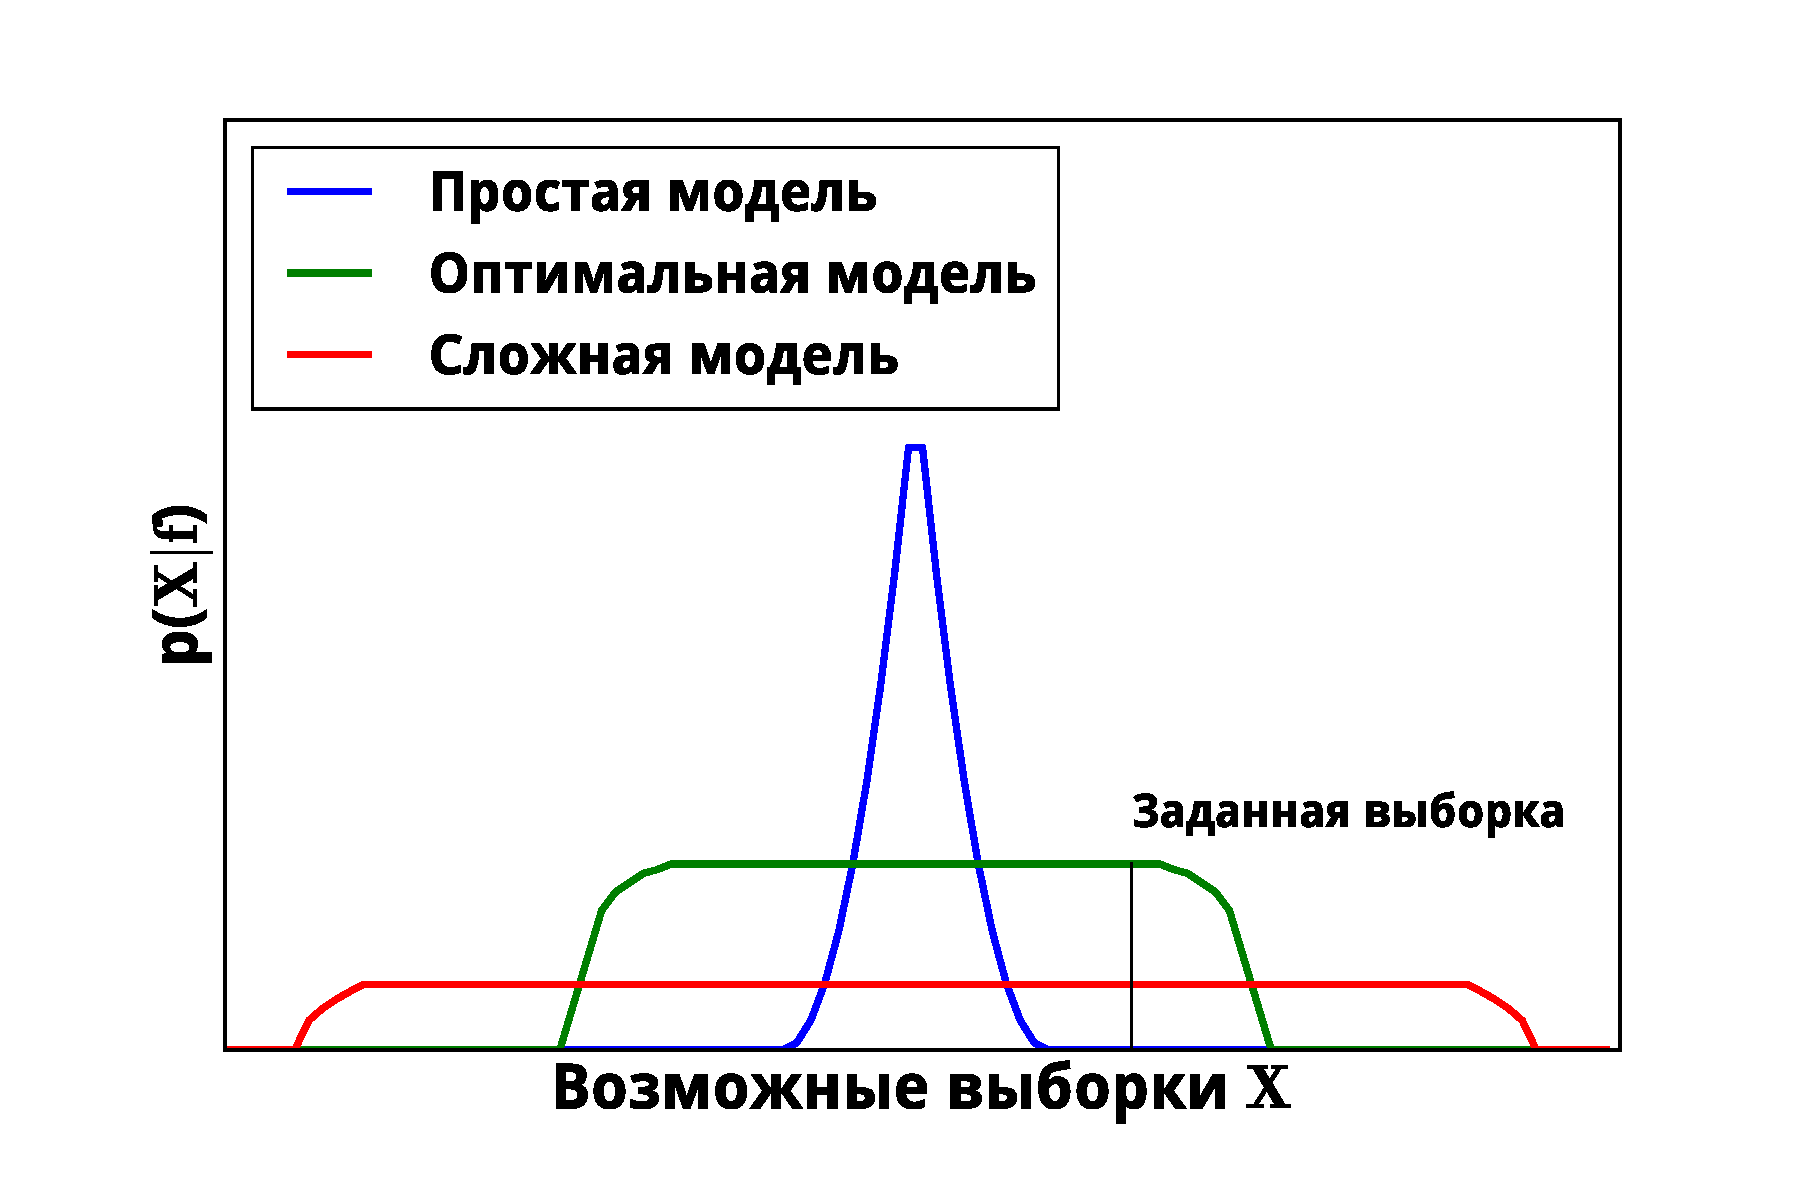
\includegraphics[width=0.4\textwidth]{evidence.pdf}} 
 \subfloat[Пример: полиномы]{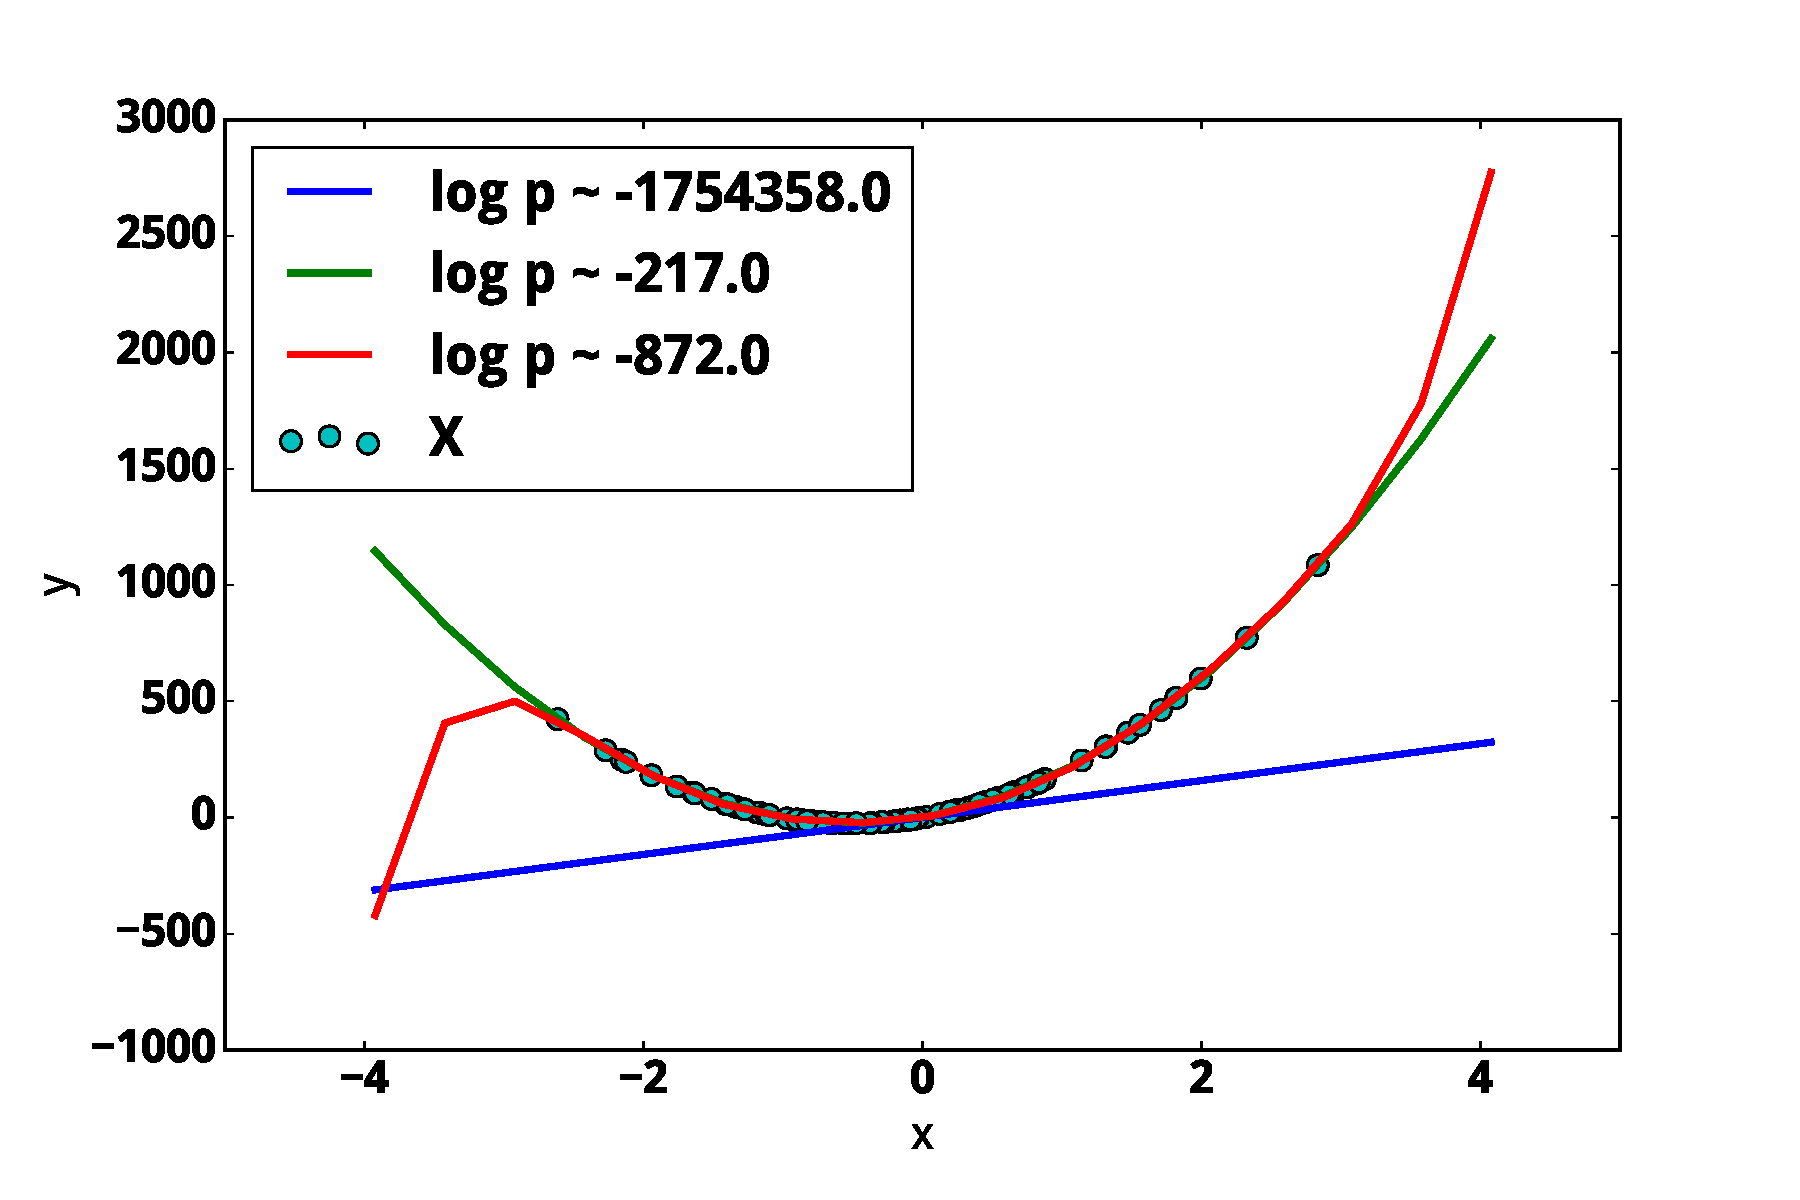
\includegraphics[width=0.4\textwidth]{example.pdf}}
\label{fig:1}\qquad

\end{figure}


\end{frame}

\begin{frame}{Evidence vs MDL}
\small
\begin{tabular}{ c | c  }
  \hline			
 \bf Evidence & \bf MDL \\
  \hline  
Использует априорные знания &  Независима от априорных знаний \\
  \hline  
Основывается на гипотезе о порождении\\ выборки & Минимизирует длину описания выборки\\ вне зависимости от их природы \\
  \hline  

\end{tabular}


\begin{figure}
  \centering
 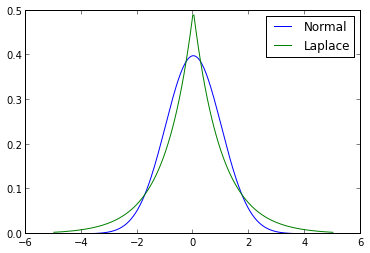
\includegraphics[width=0.4\textwidth]{laplace.png}
\label{fig:1}\qquad

\end{figure}


\end{frame}




\begin{frame}{Оптимальность модели}
\begin{block}{Определение}
Пусть задано множество моделей $M$.  \\
Пусть для каждой модели $\mathbf{f}$ задано априорное распределение параметров: $p(\mathbf{w}|\mathbf{h})$, где $\mathbf{h}$ --- параметры априорного распределения.\\
Модель $\mathbf{f}$ назовем оптимальной среди моделей ${M}$, если достигается максимум интеграла:
\[
	p(\mathfrak{D}|\mathbf{h}) = \int_\mathbf{w} p(\mathfrak{D}|\mathbf{w})p(\mathbf{w}|\mathbf{h}) d\mathbf{w}.
\]
\end{block}
\end{frame}




\section{Вариационная нижняя оценка}
\begin{frame}{Вариационная оценка, ELBO}
%http://www.orchid.ac.uk/eprints/40/1/fox_vbtut.pdf
\textbf{Вариационная оценка Evidence}, Evidence lower bound --- метод нахождения приближенного значения аналитически невычислимого распределения $p(\mathbf{w}|\mathfrak{D}, \mathbf{h})$ распределением $q(\mathbf{w}) \in \mathfrak{Q}$. Получение вариационной нижней оценки обычно сводится к задаче минимизации
$$\text{KL}(q(\mathbf{w})||p(\mathbf{w}| \mathfrak{D}))=
-\int_{\mathbf{w}} q(\mathbf{w}) \text{log}~\frac{p(\mathbf{w}| \mathfrak{D})} {q(\mathbf{w})}d\mathbf{w} = \textcolor{blue}{\mathsf{E}_{\mathbf{w}} p(\mathfrak{D}|\mathbf{w})} - \textcolor{red}{\text{KL}(q(\mathbf{w})||p(\mathbf{w}| \mathbf{h}))}.
$$

\begin{figure}
  \centering
  \subfloat[Вариационный вывод и expectation propogation (Bishop)]{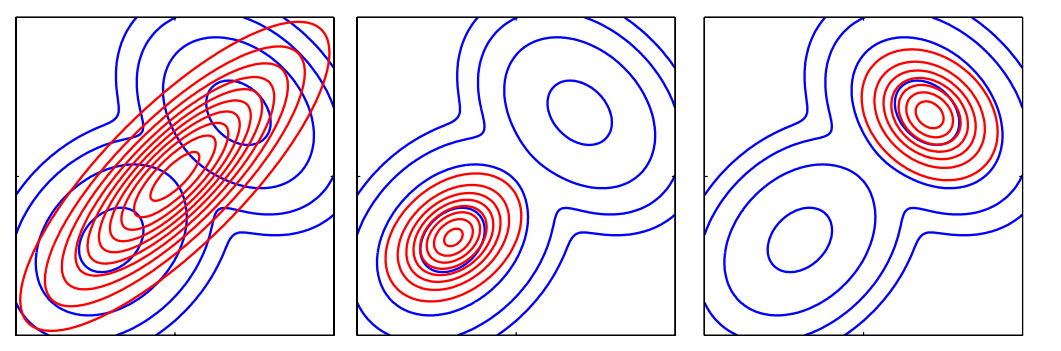
\includegraphics[width=0.66\textwidth]{bishop.png}} 
 \subfloat[{Аппроксимация Лапласа} и {вариационная оценка, зеленая линия}  (Bishop)]{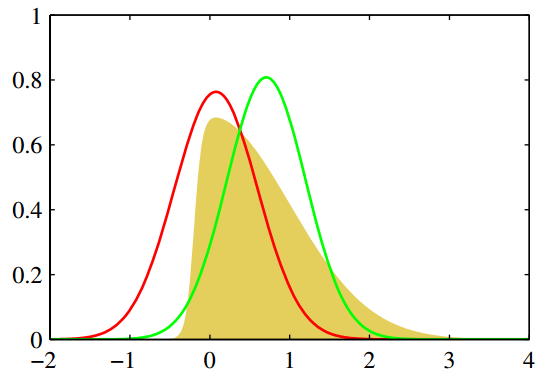
\includegraphics[width=0.33\textwidth]{laplace_vs_var.png}}
\label{fig:1}\qquad

\end{figure}

\end{frame}


\begin{frame}{Получение вариацонной нижней оценки}
\small
\begin{block}{Утверждение 1} Максимизация вариационной нижней оценки $$\int_{\mathbf{w}} q(\mathbf{w})\textnormal{log}~\frac{p(\mathbf{y},\mathbf{w}|\mathbf{X},\mathbf{h})}{q(\mathbf{w})}d\mathbf{w}$$   эквивалентна минимизации расстояния Кульбака--Лейблера между распределением $q(\mathbf{w}) \in \mathfrak{Q}$ и апостериорным распределением параметров $p(\mathbf{w}|\mathbf{y}, \mathbf{X}, \mathbf{h})$:
\[
    \hat{q} = \argmax_{q \in \mathfrak{Q}} \int_{\mathbf{w}} q(\mathbf{w})\textnormal{log}~\frac{p(\mathbf{y},\mathbf{w}|\mathbf{X},\mathbf{h})}{q(\mathbf{w})}d\mathbf{w} \Leftrightarrow 	
    \hat{q} = \argmin_{q \in  \mathfrak{Q}} \textnormal{D}_\textnormal{KL}  \bigl(q(\mathbf{w})||p(\mathbf{w}|\mathbf{y}, \mathbf{X}, \mathbf{h})\bigr),
\]
\[
	\textnormal{D}_\textnormal{KL}  \bigl(q(\mathbf{w})||p(\mathbf{w}|\mathbf{y}, \mathbf{X}, \mathbf{h})\bigr) =  \int_\mathbf{w} q(\mathbf{w}) \log \left(\frac{q(\mathbf{w})}{p(\mathbf{w}|\mathbf{y}, \mathbf{X}, \mathbf{h})}\right) d\mathbf{w}.
\]

\end{block}


\begin{block}{Определение} Модель $\mathbf{f}$ назовем субоптимальной на множестве моделей $M$, если модель доставляет максимум нижней вариационной оценке:
\[
 \int_{\mathbf{w}} q(\mathbf{w})\textnormal{log}~\frac{p(\mathbf{y},\mathbf{w}|\mathbf{X},{\mathbf{h})}}{q(\mathbf{w})}d\mathbf{w}.
\]
\end{block}


\end{frame}

\begin{frame}{Вариационная оценка и эффективный размер выборки}
\begin{block}{Утверждение 2}
Пусть $m \gg 0$, $\lambda > 0, \frac{m}{\lambda}   \in \mathbb{N}, \frac{m}{\lambda}  \gg 0.$ Тогда оптимизация функции
\[
\textcolor{blue}{\mathsf{E}_{q} \log \text{log} p(\mathbf{y}|\mathbf{X}, \mathbf{w})} - \textcolor{red}{\lambda \textnormal{D}_\textnormal{KL}  \bigl(q(\mathbf{w})||p(\mathbf{w}|\mathbf{y}, \mathbf{X}, \mathbf{h})\bigr)}
\]
 эквивалентна оптимизации вариационной оценки обоснованности  
для произвольной случайной подвыборки $\hat{\mathbf{y}}, \hat{\mathbf{X}}$ мощности $\frac{m}{{\lambda}}$ из генеральной совокупности.
\end{block}

См. также [Alemi et al., 2017, Fixing Broken ELBO].
\end{frame}

\begin{frame}{Plate notation}
Plate notation --- формат представления вероятностных моделей, альтернативный вероятностным графам.

Элементы:
\begin{itemize}
\item Белые кружки (случайные величины);
\item Серые кружки (наблюдаемые реализации случайной величины);
\item Маленькие кружки (неслучайные величины);
\item Плитки (дублирование вероятностного вывода).
\end{itemize}


\begin{figure}
  \centering
  \subfloat[DAG и Plate notation (Bishop)]{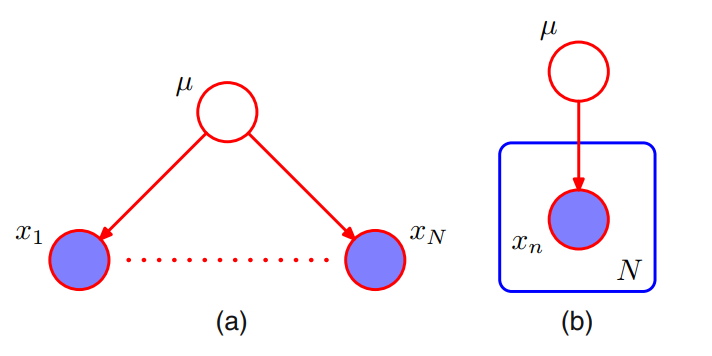
\includegraphics[width=0.38\textwidth]{dag.png}} 
 \subfloat[Plate notation для модели регрессии (Bishop)]{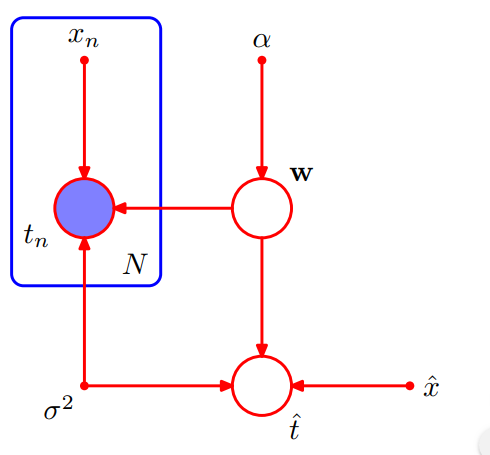
\includegraphics[width=0.35\textwidth]{poly.png}}
\label{fig:1}\qquad
\end{figure}
\end{frame}

\begin{frame}{Вариационный автокодировщик}
\begin{columns}[T]
\begin{column}{.65\textwidth}
Пусть объекты выборки $\mathbf{X}$ порождены при условии скрытой переменной $\mathbf{h} \sim \mathcal{N}(\mathbf{0}, \mathbf{I})$:
$$
\mathbf{x} \sim p(\mathbf{x}|\mathbf{h}, \mathbf{w}).
$$
$p(\mathbf{h}|\mathbf{x}, \mathbf{w})$ --- неизвестно.

Будем максимизировать вариационную оценку правдоподобия выборки:
$$
\text{log}p(\mathbf{x}|\mathbf{w}) \geq \mathsf{E}_{q_\phi(\mathbf{h}|\mathbf{x})}\text{log}~p(\mathbf{x}|\mathbf{h}, \mathbf{w}) - D_\text{KL}(q_\phi(\mathbf{h}|\mathbf{x})||p(\mathbf{h})) \to \max.
$$

Распределения $q_\phi(\mathbf{h}|\mathbf{x})$ и $p(\mathbf{x}|\mathbf{h}, \mathbf{w})$ моделируются нейросетью:
$$
q_\phi(\mathbf{h}|\mathbf{x}) \sim \mathcal{N}(\boldsymbol{\mu}_\phi(\mathbf{x}),\boldsymbol{\sigma}_\phi^2(\mathbf{x})), 
$$
$$
p(\mathbf{x}|\mathbf{h}, \mathbf{w}) \sim \mathcal{N}(\boldsymbol{\mu}_w(\mathbf{h}),\boldsymbol{\sigma}_w^2(\mathbf{h})),
$$
где функции $\boldsymbol{\mu}$,$\boldsymbol{\sigma}$ --- выходы нейросети.\\
\end{column}%
\hfill%
\begin{column}{.25\textwidth}
\begin{figure}
  \centering
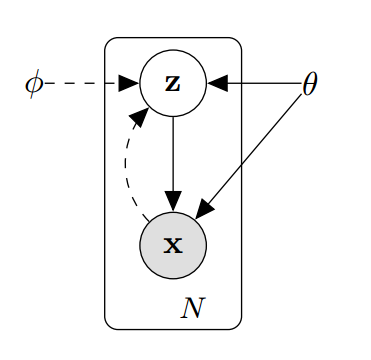
\includegraphics[width=\textwidth]{graph.png}
\end{figure}
\end{column}
\end{columns}
\end{frame}




\begin{frame}{Использование вариационной нижней оценки}
\textbf{Для чего используют вариационный вывод?}
\begin{itemize}
\item получение оценок Evidence;
\item получение оценок распределений моделей со скрытыми переменными (тематическое моделирование, снижение размерности).
\end{itemize}

\textbf{Зачем используют вариационный вывод?}
\begin{itemize}
\item сводит задачу нахождения апостериорной вероятности к методам оптимизации;
\item проще масштабируется, чем аппроксимация Лапласа;
\item проще в использовании, чем сэмплирующие методы.
\end{itemize}
\textbf{Вариационный вывод может давать сильно заниженную оценку.}
\end{frame}


\section{Получение оценок для разделяющих моделей}
\begin{frame}{ELBO: нормальное распределение}
Пусть $q \sim \mathcal{N}(\boldsymbol{\mu}_q, \mathbf{A}_q).$\\
Тогда вариационная оценка имеет вид:
$$
\textcolor{blue}{\int_{\mathbf{w}} q(\mathbf{w})\text{log}~{p(\mathbf{Y}|\mathbf{X},\mathbf{w},\mathbf{h})} d \mathbf{w}} - \textcolor{red}{D_\text{KL}\bigl(q (\mathbf{w} )|| p (\mathbf{w}|\mathbf{h})\bigr)} \simeq
$$
$$
\textcolor{blue}{\sum_{i=1}^m \text{log}~p(\mathbf{y}_i|\mathbf{x}_i, \hat{\mathbf{w}})} - \textcolor{red}{D_\text{KL}\bigl(q (\mathbf{w} )|| p (\mathbf{w}|\mathbf{h})\bigr)} \to \max_{\mathbf{A}_q, \boldsymbol{\mu}_q}, \quad \hat{\mathbf{w}} \sim q.
$$
В случае, если априорное распределение параметров $p(\mathbf{w}|\mathbf{h})$ является нормальным: 
$$
p(\mathbf{w}|\mathbf{h}) \sim \mathcal{N}(\boldsymbol{\mu}, \mathbf{A}),
$$
дивергенция $D_\text{KL}\bigl(q (\mathbf{w} )|| p (\mathbf{w}|\mathbf{h})$ вычисляется аналитически:
$$
 \textcolor{red}{D_\text{KL}\bigl(q (\mathbf{w}) || p (\mathbf{w}|\mathbf{h})\bigr)} = \frac{1}{2} \bigl( \text{tr} (\mathbf{A}^{-1}\mathbf{A}_q) + (\boldsymbol{\mu} - \boldsymbol{\mu}_q)^\text{T}\mathbf{A}^{-1}(\boldsymbol{\mu} - \boldsymbol{\mu}_q) - n +\text{ln}~|\mathbf{A}| - \text{ln}~|\mathbf{A}_q| \bigr).
$$
\end{frame}



\begin{frame}
\frametitle{ Graves, 2011}


\textbf{Априорное распределение:} $p(\mathbf{w}|\sigma) \sim \mathcal{N}(\boldsymbol{\mu}, \sigma \mathbf{I}).$\\
\textbf{Вариационное распределение:} $q (\mathbf{w}) \sim \mathcal{N}(\boldsymbol{\mu}_q, \sigma_q \mathbf{I}).$\\
Жадная оптимизация гиперпараметров:
\[
	\boldsymbol{\mu} = \hat{\mathsf{E}} \mathbf{w},
\quad
	\sigma = \hat{\mathsf{D}} \mathbf{w}.
\]

Прунинг параметра ${w}_i$ определяется относительной плотностью:
\[
	\lambda = \frac{q(\mathbf{0})}{q(\boldsymbol{\mu}_{i,q})}  = \text{exp}(-\frac{\mu_i^2}{2\sigma_i^2}).
\]
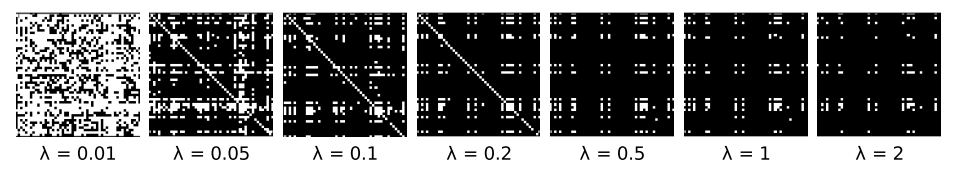
\includegraphics[width=\textwidth]{graves.png}
\end{frame}



\begin{frame}{ELBO: нормальное распределение}
\begin{columns}[T] 
\begin{column}{.48\textwidth}
\textbf{``Обычная'' функция потерь:}\\
$$
L = \textcolor{blue}{\sum_{\mathbf{x}, \mathbf{y} \in \mathfrak{D}} - \text{log}p(\mathbf{y}|\mathbf{x}, \mathbf{w})} + \textcolor{red}{\lambda||\mathbf{w}||_2^2}.
$$\\~\\

% если n - константна.
\textbf{Вариационный вывод при $(p(\mathbf{w}|\mathbf{h}) \sim \mathcal{N}(\mathbf{0}, \mathbf{1}))$:}\\
$$
L =   \textcolor{blue}{\sum_{\mathbf{x}, \mathbf{y}} \text{log}~p(\mathbf{y}|\mathbf{x}, \hat{\mathbf{w}})} +
$$
$$ + \textcolor{red}{\frac{1}{2} \bigl( \text{tr} (\mathbf{A}_q) + \boldsymbol{\mu}_q^\text{T}\mathbf{A}^{-1}\boldsymbol{\mu}_q  - \text{ln}~|\mathbf{A}_q| \bigr)}.
$$\\~\\

\end{column}%
\hfill%
\begin{column}{.48\textwidth}

\begin{center}
\begin{figure}
\caption*{Пример грубой аппроксимации нормальным диагональным распределением $q$}
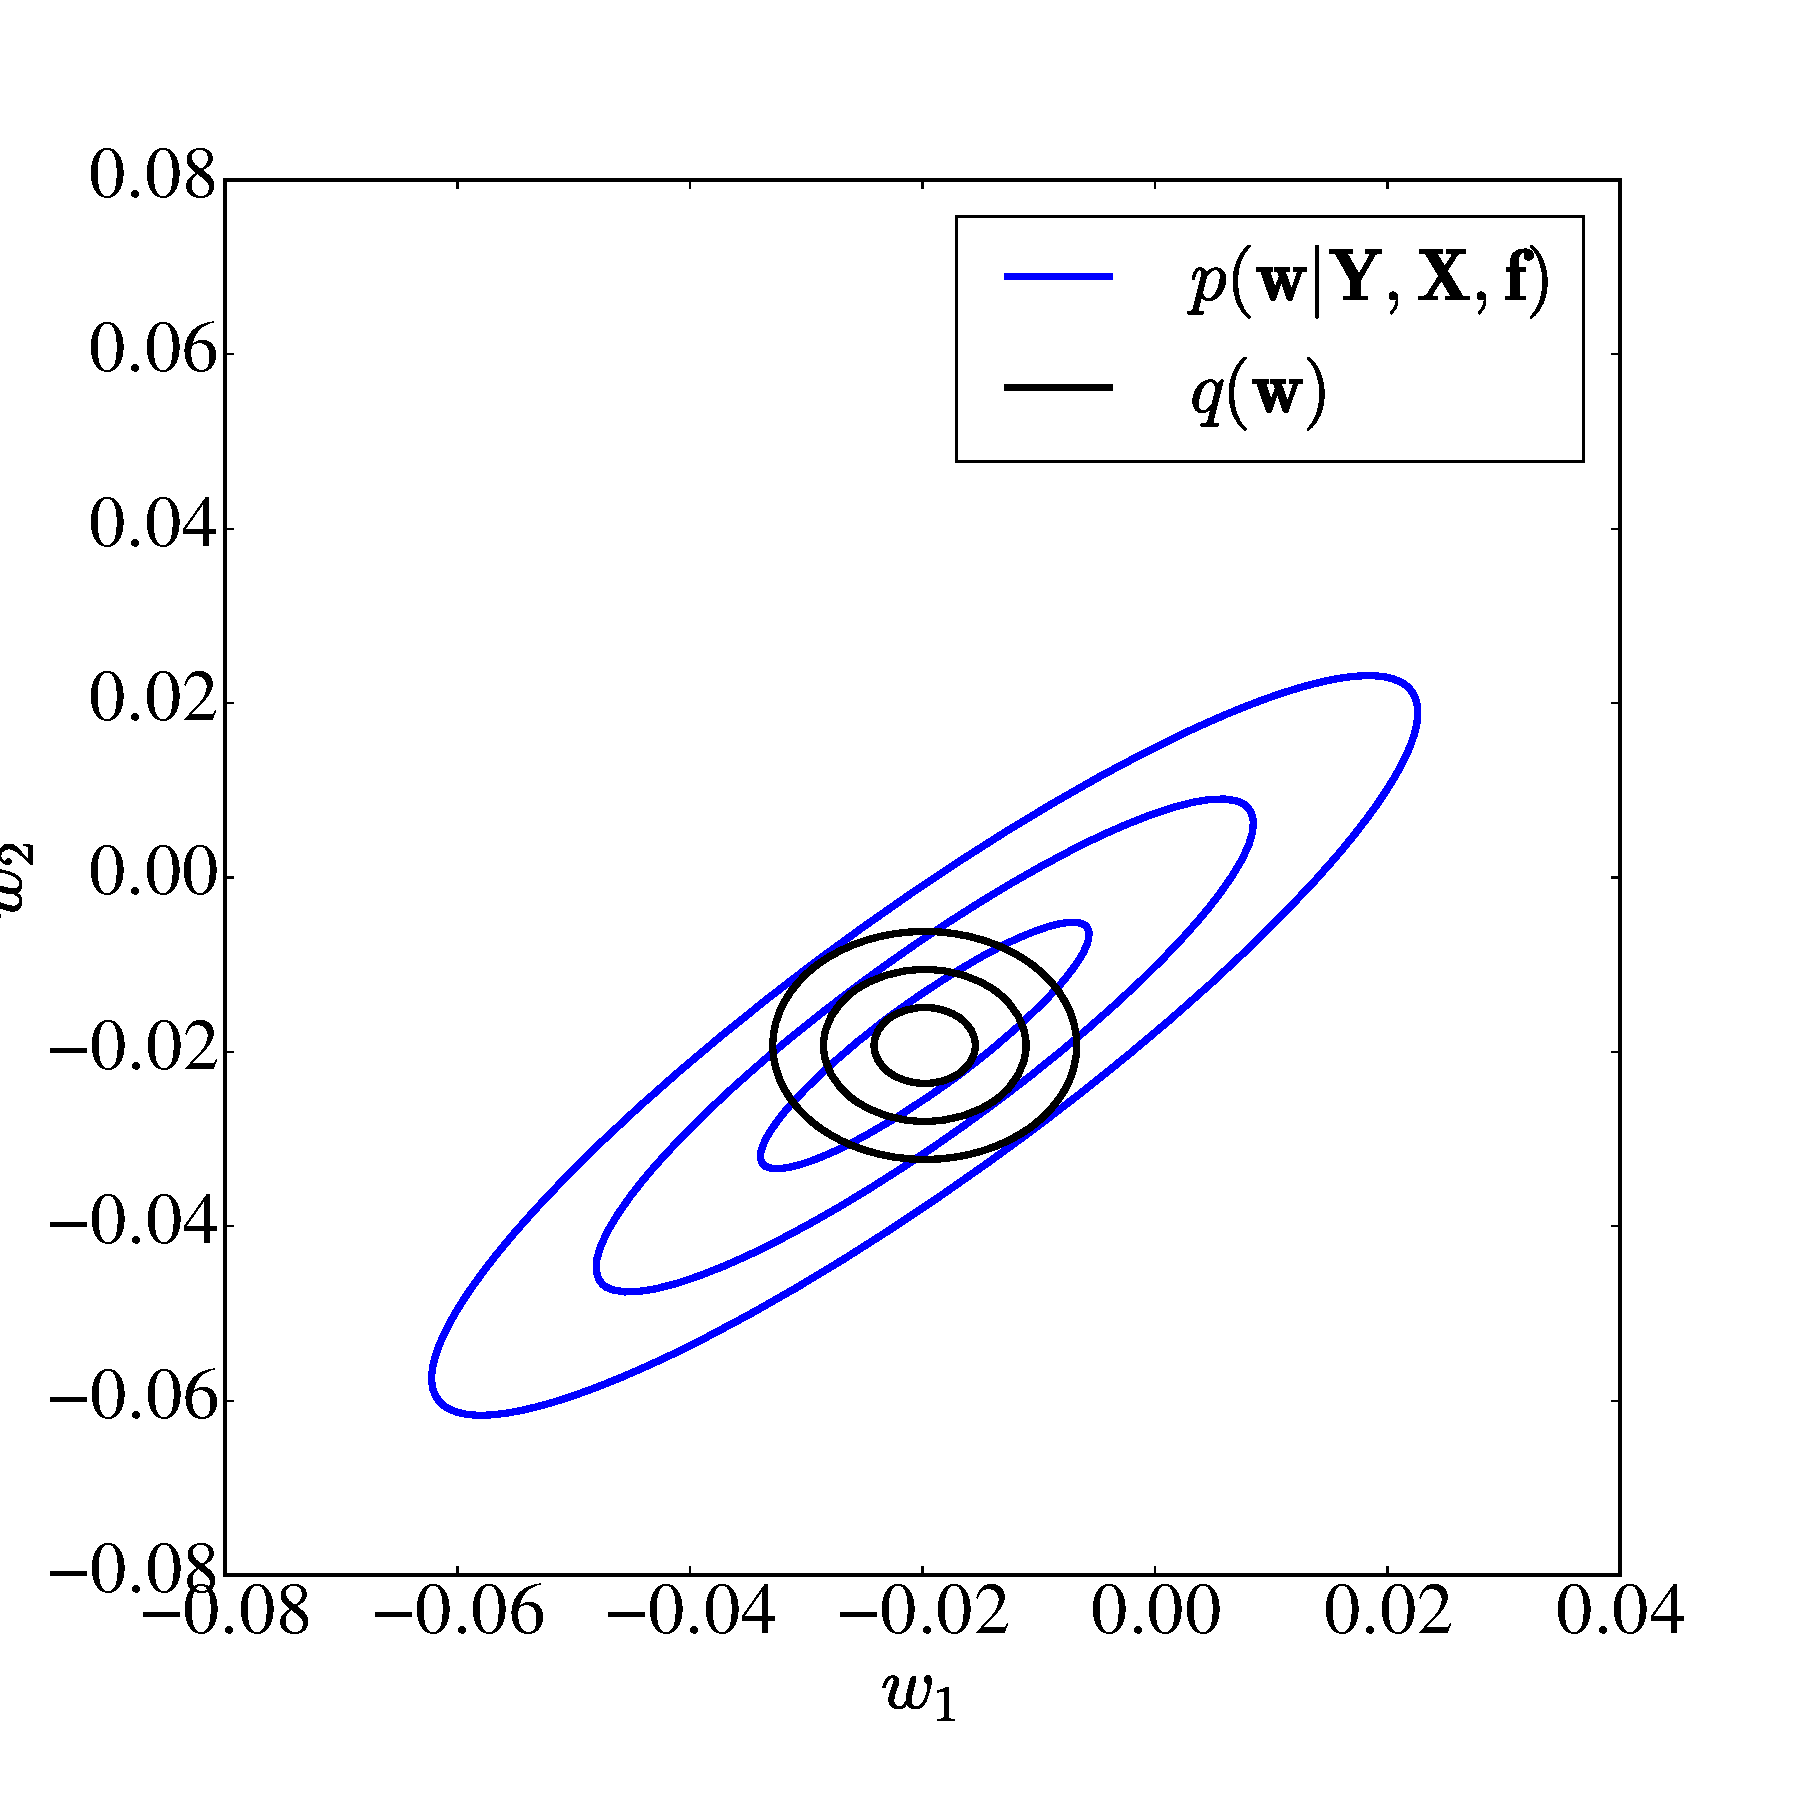
\includegraphics[width=0.8\textwidth]{mf.pdf}
\end{figure}
\end{center}

\end{column}%
\end{columns}

\end{frame}







\begin{frame}{MCMC и вариационный вывод}
\textbf{Идея MCMC:}
Порождаем сэмплы из простого распределения и принимаем их, если заданное отношение больше порога:
\[
    \min\left(1, \frac{p(\mathbf{w}^{\tau}|\mathbf{y}, \mathbf{X}, \mathbf{h})}{p(\mathbf{w}^{\tau - 1}|\mathbf{y}, \mathbf{X}, \mathbf{h})}\right),
\]
где $\mathbf{w}^{\tau}$ выбирается на основе предыдущего сэмпла:
\[
    \mathbf{w}^{\tau} = T(\mathbf{w}^{\tau - 1}).
\]

\textbf{Salimans et al., 2014:} будем интерпретировать последовательность применения оператора $T$ как оптимизацию вариационной оценки:
\[
    T^1 \circ \dots T^\eta(\mathbf{w}) \to p(\mathbf{w}^{\tau}|\mathbf{y}, \mathbf{X}, \mathbf{h}).
\]

\textbf{Maclaurin et. al, 2015:}  в качестве оператора $T$ будем рассматривать оператор оптимизации. Откажемся от отклонения сэмплов по порогу.
\end{frame}


\begin{frame}{Оператор оптимизации, Maclaurin et. al, 2015}
\begin{block}{Определение}
Назовем оператором оптимизации алгоритм $T$ выбора вектора параметров $\mathbf{w}'$  по параметрам предыдущего шага $\mathbf{w}$:
\[
	\mathbf{w}' = T(\mathbf{w}).
\]
\end{block}

\begin{block}{Определение}
Пусть $L$ --- дифференцируемая функция потерь. \\
Оператором градиентного спуска назовем следующий оператор:
\[
    T(\mathbf{w}) = \mathbf{w} - \beta \nabla L(\mathbf{w}, \mathbf{y}, \mathfrak{D}).
\]
\end{block}


\end{frame}

\begin{frame}{Градиентный спуск для оценки правдоподобия}
Рассмотрим максимизацию совместного распределения параметров:
\[
    L =  -\text{log}~p(\mathfrak{D},\mathbf{w}|\mathbf{h}) = -\sum_{\mathfrak{D} \in \mathfrak{D}} \text{log}~p(\mathfrak{D}|\mathbf{w}, \mathbf{h}) p(\mathbf{w}|\mathbf{h})
\]
Проведем оптимизацию нейросети  из $r$ различных начальных приближений $\mathbf{w}_1, \dots, \mathbf{w}_r$ с использованием градиентного спуска:
\[
\mathbf{w}' = T(\mathbf{w}).
\]

Векторы параметров $\mathbf{w}_1,\dots,\mathbf{w}_r$ соответствуют некоторому скрытому распределению $q(\mathbf{w})$.

\end{frame}



\begin{frame}{Энтропия}
Формулу вариационной оценки можно переписать с использованием энтропии:
$$\text{log}~p(\mathfrak{D}|\mathbf{f}) \geq 
\int_{\mathbf{w}} q(\mathbf{w})\text{log}~\frac{p(\mathfrak{D},\mathbf{w}|\mathbf{h})}{q(\mathbf{w})}d\mathbf{w} = 
$$
$$
\mathsf{E}_{q(\mathbf{w)}}[\text{log~}p (\mathfrak{D}, \mathbf{w}| \mathbf{h})] + \mathsf{S}({q(\mathbf{w)}}),
$$
где $\mathsf{S}({q(\mathbf{w)}})$ --- энтропия:
$$
\mathsf{S}({q(\mathbf{w)}}) = - \int_{\mathbf{w}} q(\mathbf{w})\text{log}~q(\mathbf{w})d\mathbf{w}.  	
$$
\end{frame}


\begin{frame}{Градиентный спуск для оценки правдоподобия}
\begin{block}{Утверждение 3}
Пусть $L$ --- липшицева функция, оператор оптимизации --- биекция.
Тогда разность энтропии на различных шагах оптимизации вычисляется как:
\[
\mathsf{S}(q'(\mathbf{w})) -  \mathsf{S}(q(\mathbf{w}))  \simeq  \frac{1}{r}\sum_{g=1}^r \bigl(-\beta \text{Tr}[\mathbf{H}(\mathbf{w}'^g)] - \beta^2 \text{Tr}[\mathbf{H}(\mathbf{w}'^g)\mathbf{H}(\mathbf{w}'^g)]  \bigr).
\]
\end{block}

Итоговая оценка на шаге оптимизации $\tau$:
$$
\text{log}~\hat{p}(\mathbf{Y}|\mathfrak{D}, \mathbf{h}) \sim \frac{1}{r} \sum_{g = 1}^r L(\mathbf{w}^g_\tau, \mathfrak{D}, \mathbf{Y})  + \mathsf{S}(q^0(\mathbf{w}))+$$ $$ + \frac{1}{r}\sum_{b=1}^\tau\sum_{g=1}^r \bigl(-\beta \text{Tr}[\mathbf{H}(\mathbf{w}_b^g)] - \beta^2 \text{Tr}[\mathbf{H}(\mathbf{w}_b^g)\mathbf{H}(\mathbf{w}_b^g)]  \bigr),
$$
$\mathbf{w}_b^g$ --- вектор параметров старта $g$ на шаге $b$, $\mathsf{S}(q^0(\mathbf{w}))$ --- начальная энтропия.
\end{frame}
\begin{frame}{Переобучение,  Maclaurin et. al, 2015}
Градиентный спуск не минимизирует дивергенцию $\text{KL}(q(\mathbf{w})||p(\mathbf{w}| \mathfrak{D}, \mathbf{h}))$. При приближении к моде распределения снижается оценка Evidence, что интерпретируется как переоубчение модели.

\begin{figure}
  \centering
  \subfloat[Схождение распределения к моде]{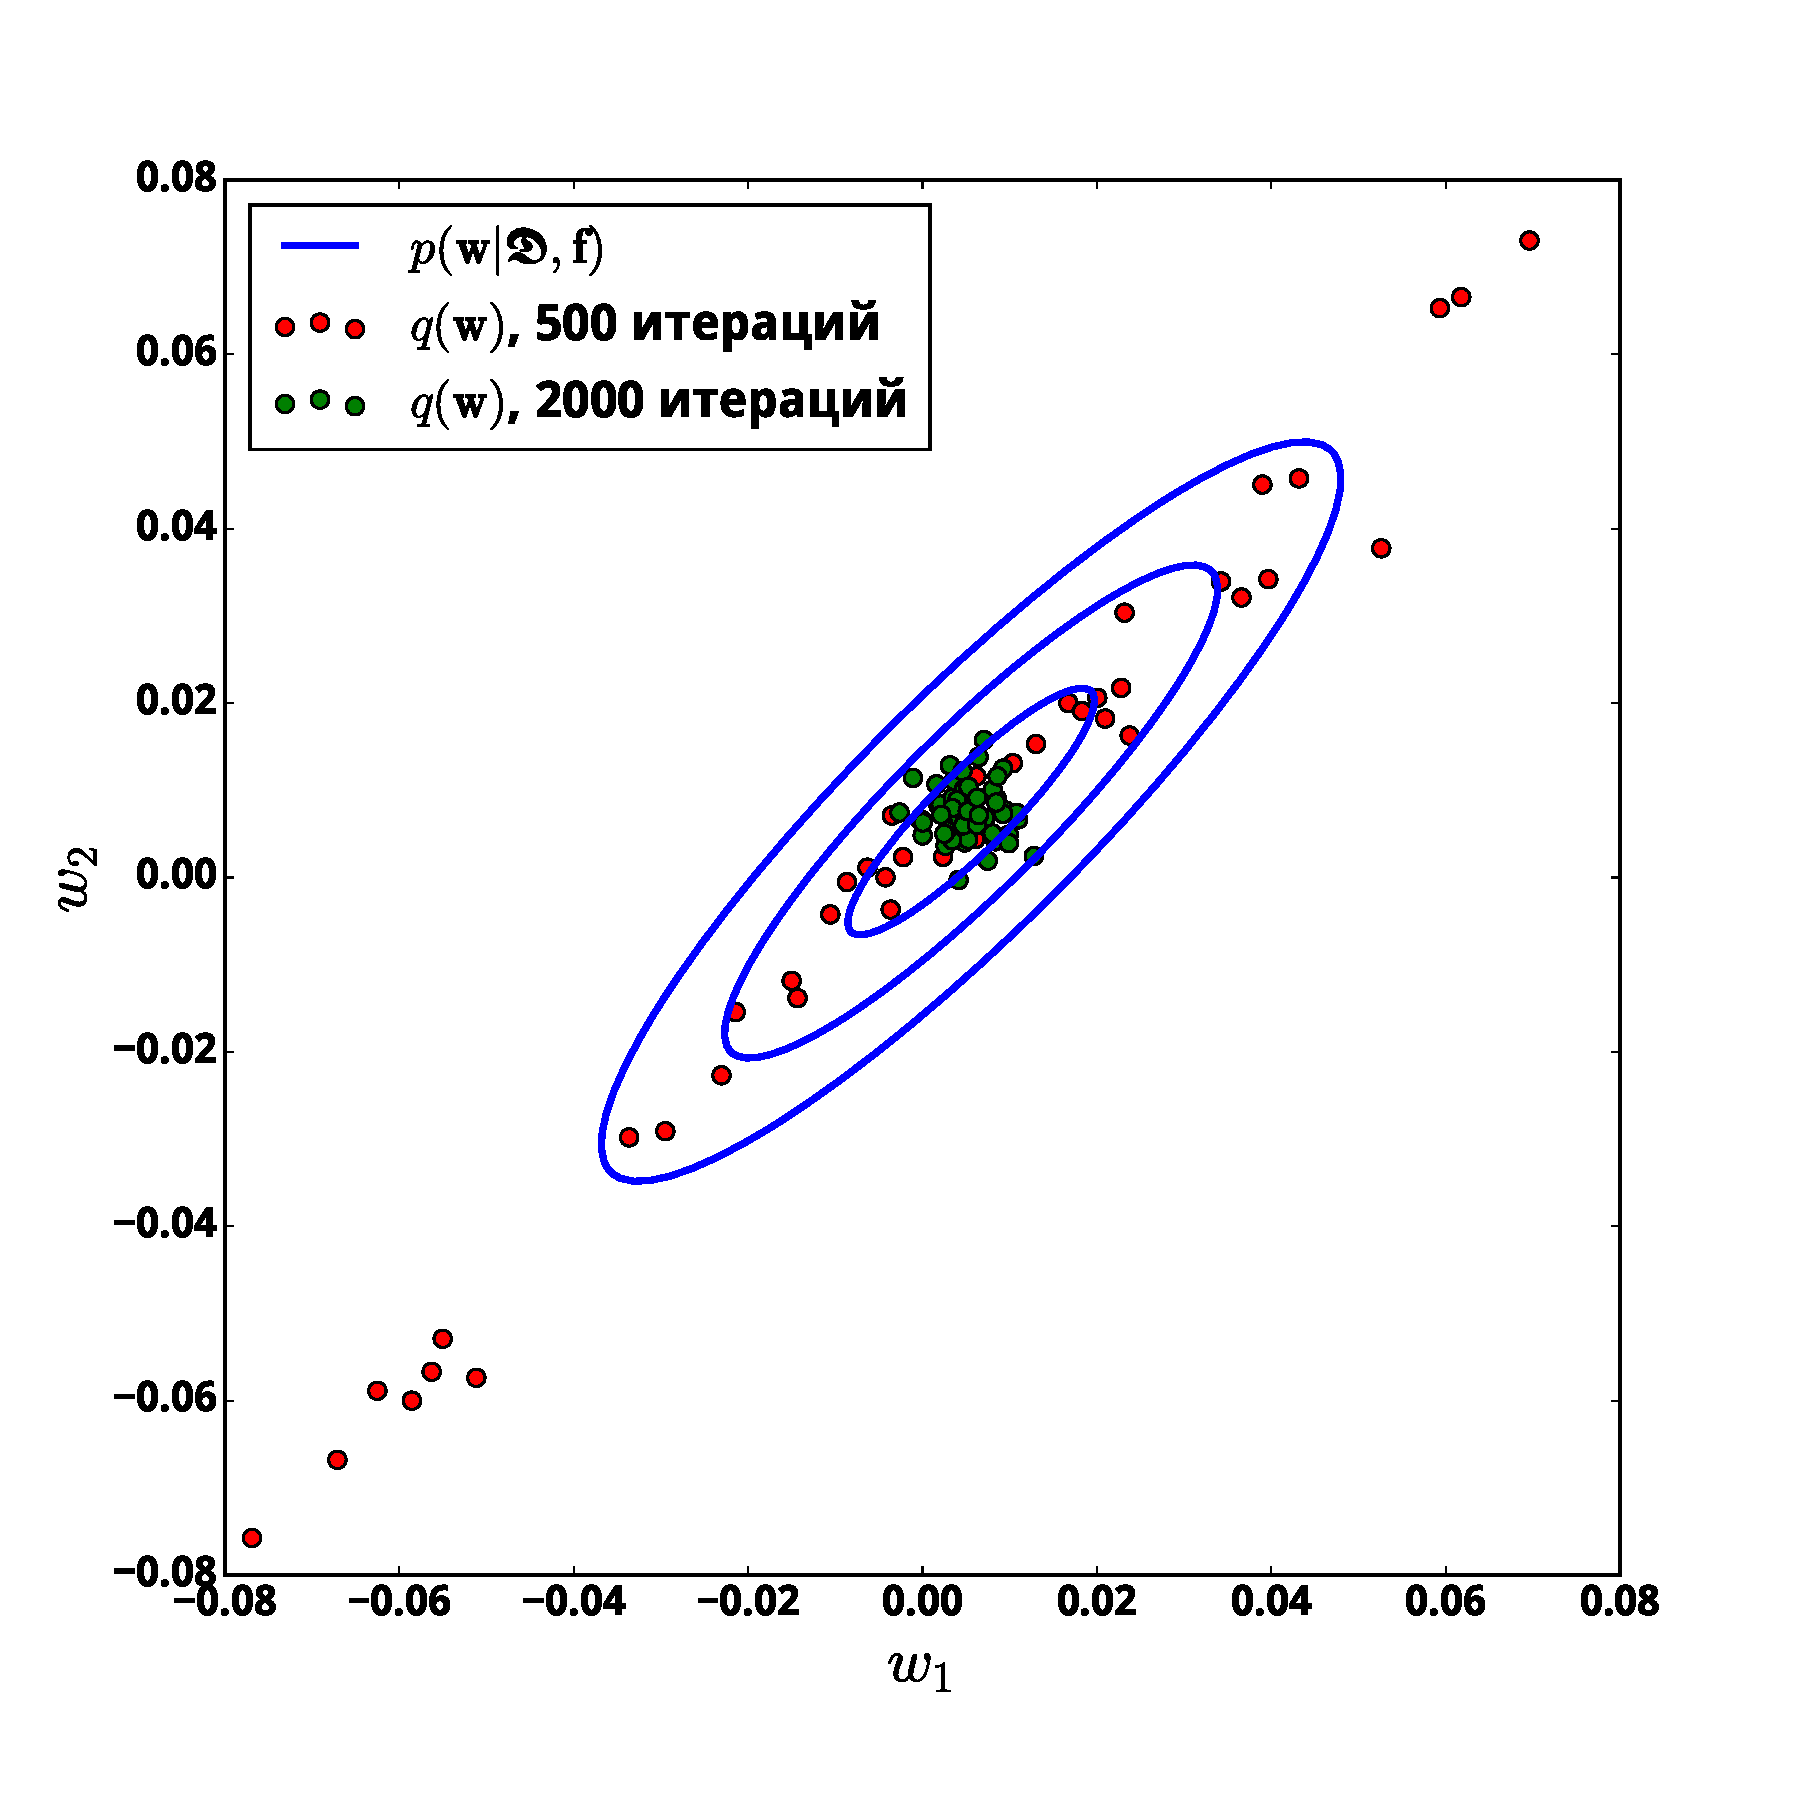
\includegraphics[width=0.35\textwidth]{sgd_estimate.pdf}} 
 \subfloat[Оценка начала переобучения]{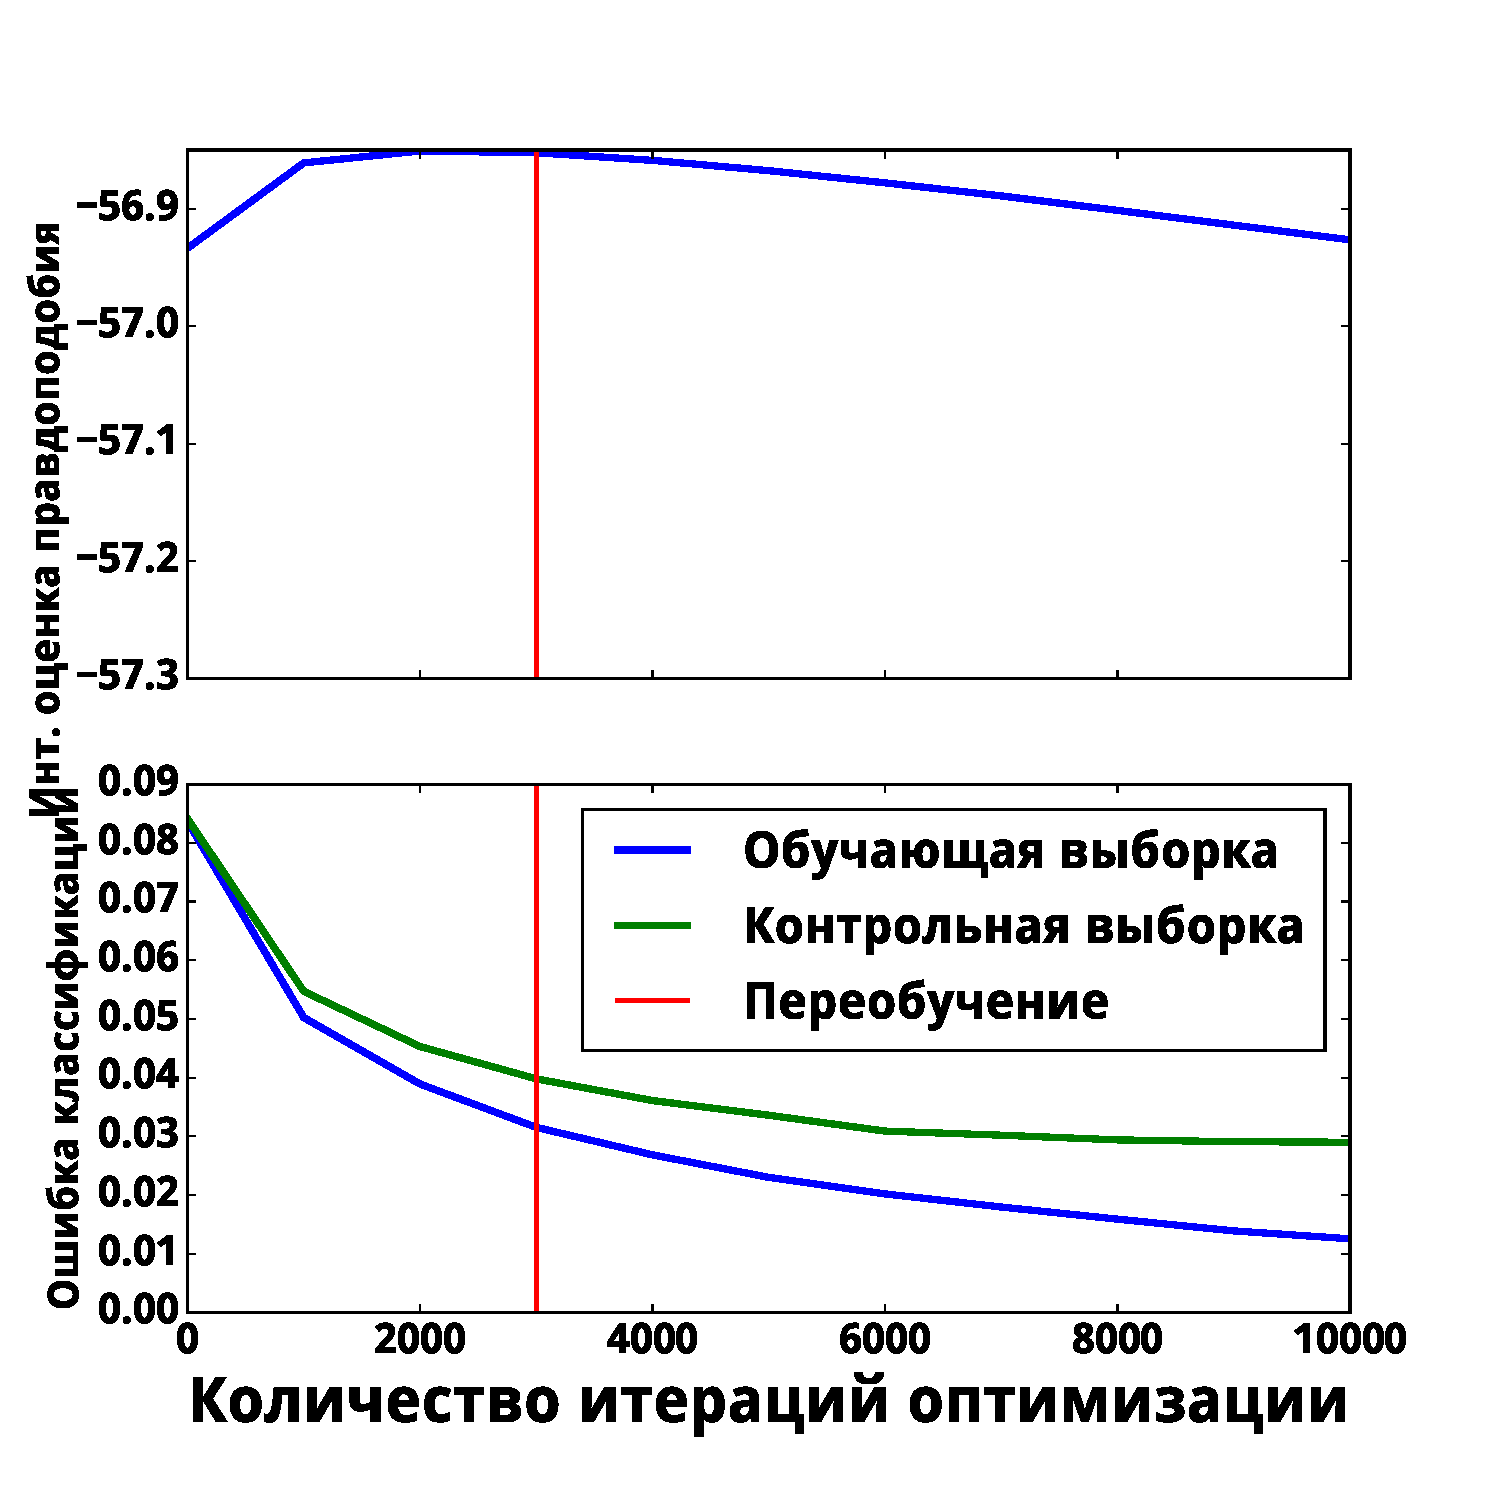
\includegraphics[width=0.35\textwidth]{sgd_show.pdf}}
\label{fig:1}\qquad
\end{figure}
\end{frame}

\begin{frame}{Стохастическая динамика Ланжевена}
Модификация стохастического градиентного спуска:
\[
	T =\mathbf{w} -  \beta  \nabla  L  \textcolor{olive}{+ \epsilon}, \quad   \textcolor{olive}{\epsilon \sim  \mathcal{N}({0},{\frac{\alpha}{2}})}
\]
где шаг оптимизации $\alpha$ изменяется с количеством итераций:
\[
	\sum_{\tau=1}^\infty \beta_\tau = \infty, \quad \sum_{\tau=1}^\infty \beta_\tau^2 < \infty.
\]
\textbf{Утверждение~[Welling, 2011].} Распределине $q^\tau(\mathbf{w})$ сходится к апостериорному распределению $p(\mathbf{w} | \mathbf{X},\mathbf{f})$.


Изменение энтропии с учетом добавленного шума:
\[
\hat{\mathsf{S}}\bigl(q^\tau(\mathbf{w})\bigr)   \geq \frac{1}{2}|\mathbf{w}|\text{log}\bigl(\text{exp}(\frac{2\mathsf{S}(q^\tau(\mathbf{w}))}{|\mathbf{w}|}) + \text{exp}(\frac{2\mathsf{S}( \epsilon)}{|\mathbf{w}|})\bigr).
\]
\end{frame}




\begin{frame}{Стохастическая динамика Ланжевена в генеративных моделях}
\textbf{Altieri et al., 2015:} будем сэмплировать скрытую переменную $\mathbf{z}$ и приближать его распределение к максимуму вариационной оценки с использованием динамики Ланжевена.
\begin{figure}[h]
\centering
\subfloat[]{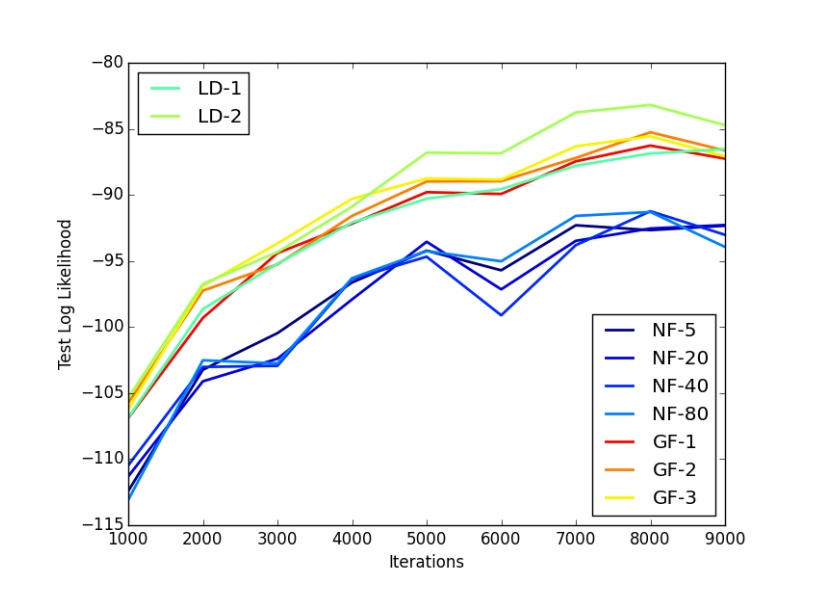
\includegraphics[width=0.65\textwidth]{./lang_original.png}}
\end{figure}
\end{frame}

\begin{frame}
\frametitle{Стохастическая динамика Ланжевена}
Распределения параметров после 2000 итераций:
\begin{figure}[h]
\centering
\subfloat[]{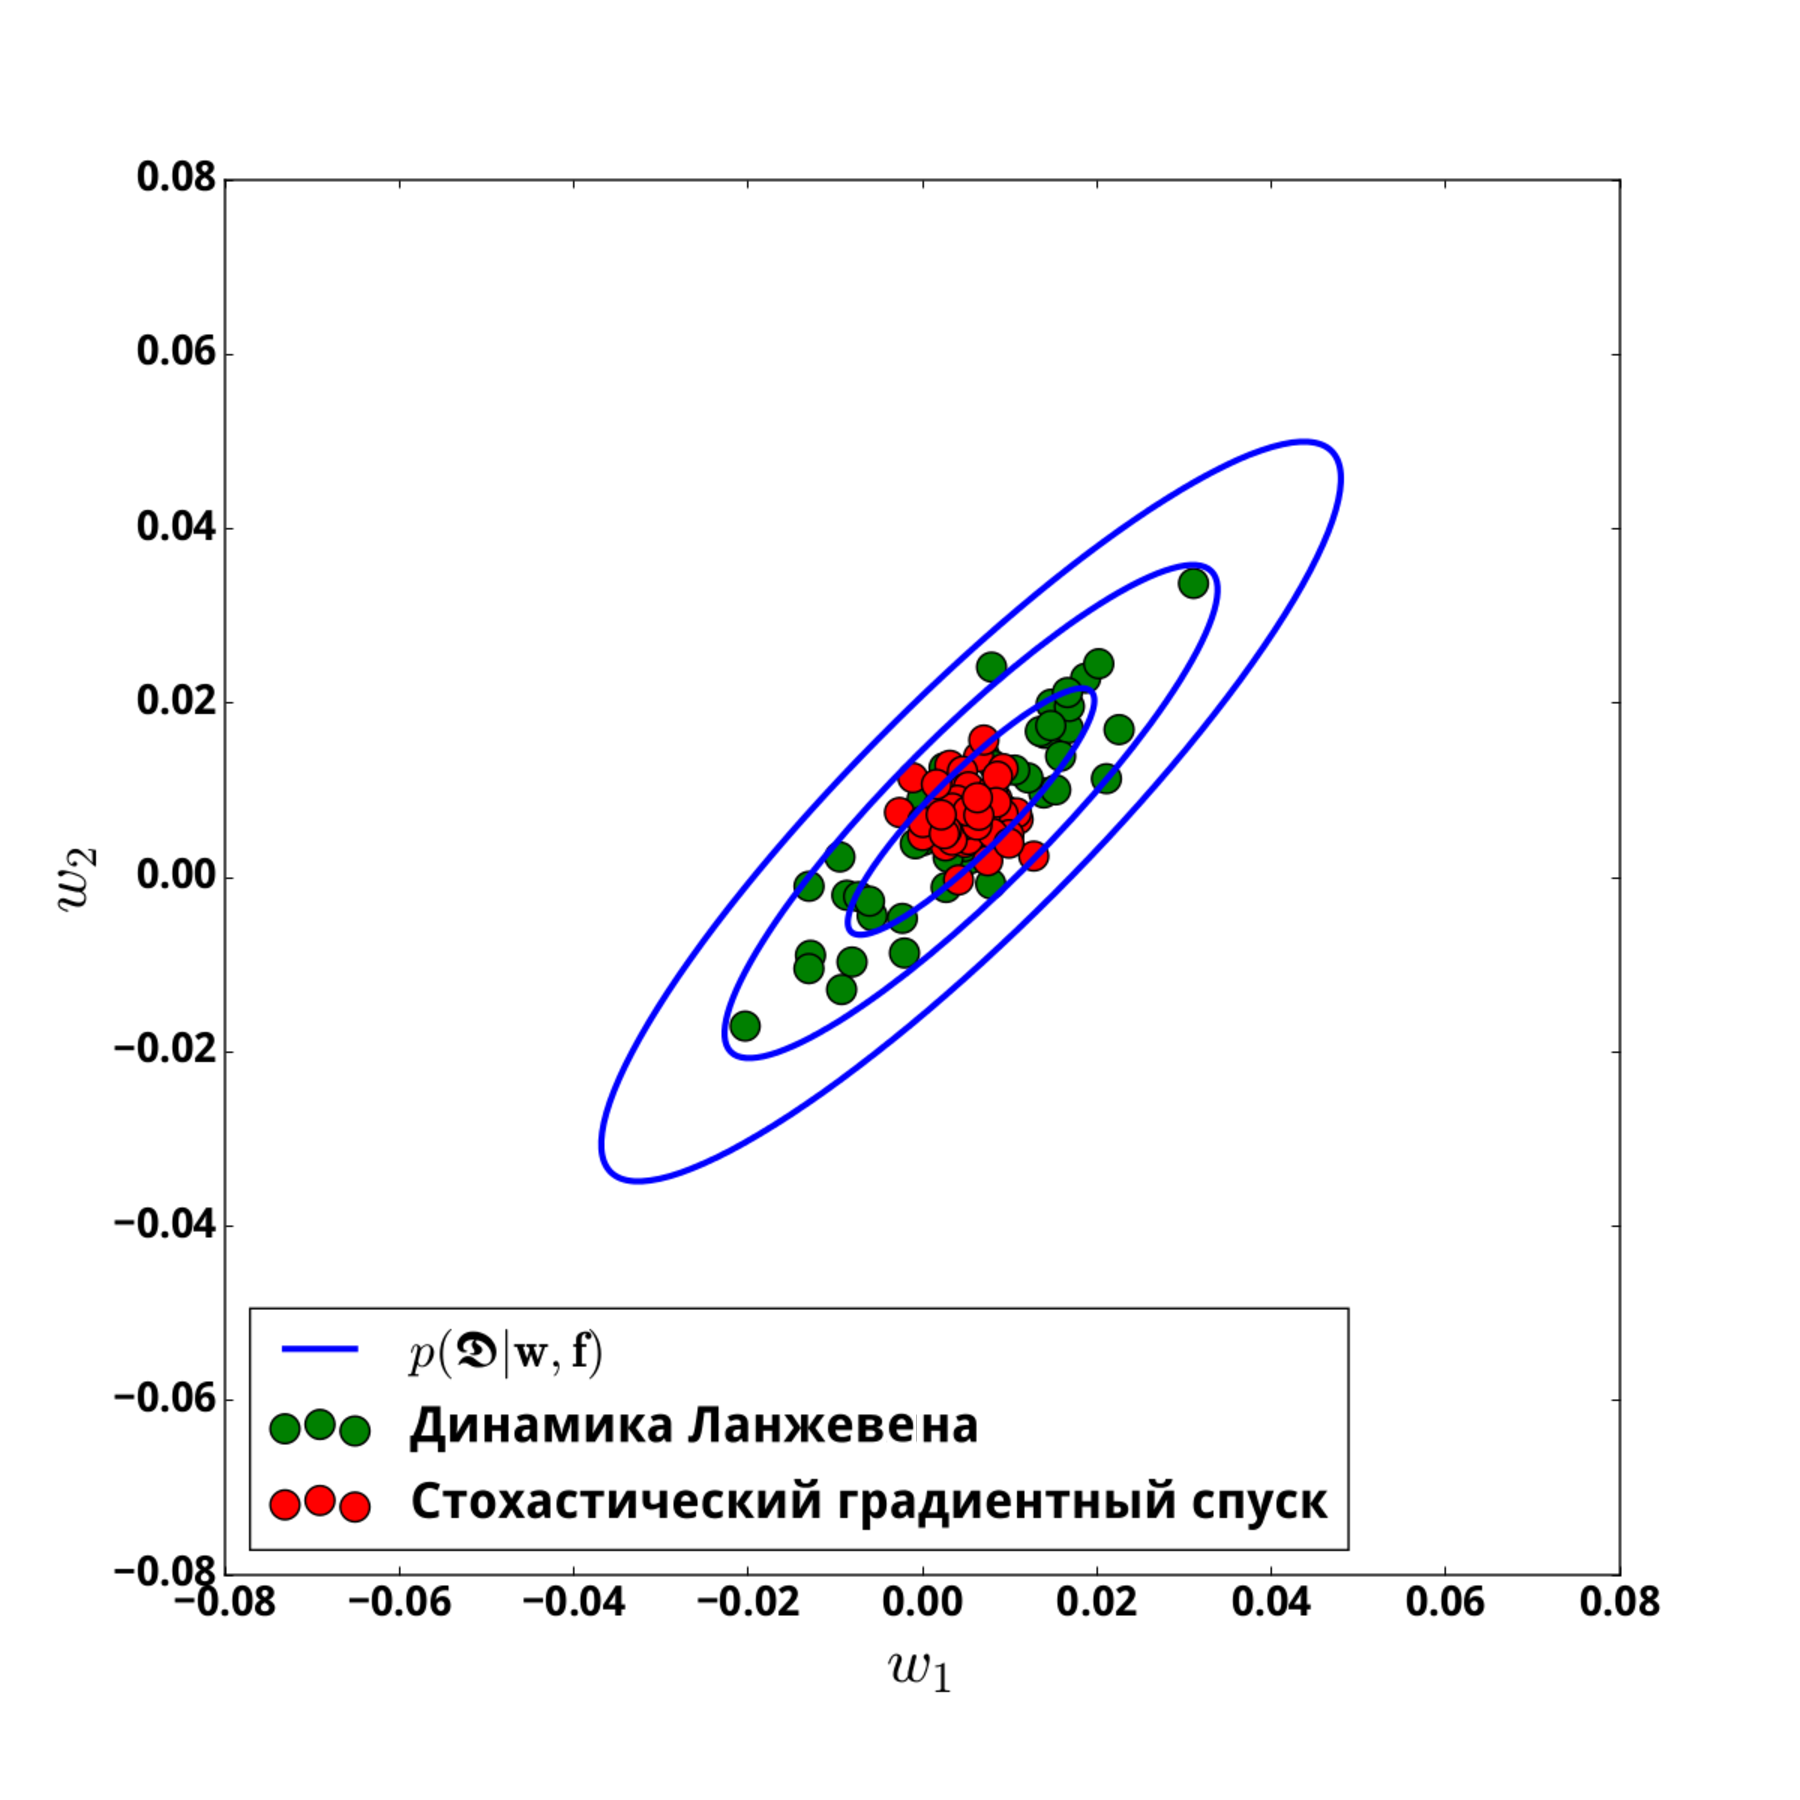
\includegraphics[width=0.45\textwidth]{./langevin_estimate.pdf}}
\end{figure}

\textbf{Проблема:} медленная сходимость динамики.

\end{frame}



\begin{frame}{SGD с оптимизацией длины шага}
\textbf{Mandt et al., 2017:} вблизи точки экстремума градиентный спуск приближает апостериорное распределение параметров модели. Существуют оценки на длину шага градиентного спуска.

\begin{figure}
  \centering
  \subfloat[SGD c разным типом длин шагов]{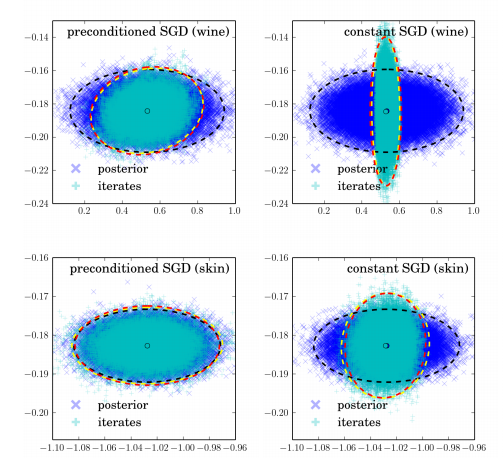
\includegraphics[width=0.45\textwidth]{blei2.png}} 
 \subfloat[Сравнение с динамикой Ланжевена]{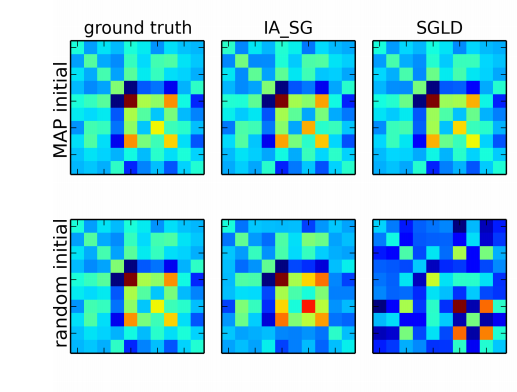
\includegraphics[width=0.45\textwidth]{blei1.png}}
\label{fig:1}\qquad
\end{figure}

\end{frame}

\begin{frame}{Список источников}
\begin{itemize}
\item Zoph, B., Vasudevan, V., Shlens, J. and Le, Q.V., 2018. Learning transferable architectures for scalable image recognition
\item David J. C. MacKay, Information Theory, Inference \& Learning Algorithms
\item Peter Grunwald, A tutorial introduction to the minimum description length principle
\item Kuznetsov M.P., Tokmakova A.A., Strijov V.V. Analytic and stochastic methods of structure parameter estimation
\item Christopher Bishop, Pattern Recognition and Machine Learning
\item Diederik P Kingma, Max Welling, Auto-Encoding Variational Bayes
\item Dougal Maclaurin, David Duvenaud, Ryan P. Adams, Early Stopping is Nonparametric Variational Inference
\item Max Welling, Yee Whye Teh, Bayesian Learning via Stochastic Gradient Langevin Dynamics
\end{itemize}
\end{frame}

\begin{frame}
\frametitle{Список источников}
\begin{itemize}
\item A. Graves, Practical Variational Inference for Neural Networks
\item Salimans, Tim, Diederik Kingma, and Max Welling, 2015. Markov chain monte carlo and variational inference: Bridging the gap
\item Altieri: http://approximateinference.org/accepted/AltieriDuvenaud2015.pdf
\item Stephan Mandt, Matthew D. Hoffman, David M. Blei, 2017. Stochastic Gradient Descent as Approximate Bayesian Inference
\item О. Ю. Бахтеев, В. В. Стрижов, “Выбор моделей глубокого обучения субоптимальной сложности”
\item А. Н. Смердов, О. Ю. Бахтеев, В. В. Стрижов, “Выбор оптимальной модели рекуррентной сети в задачах поиска парафраза”
\end{itemize}
\end{frame}

\begin{frame}{ДЗ: выбор задания}
\textbf{Дедлайн: 23 октября, 0 часов.}\\~\\

\texttt{ from zlib import crc32}\\~\\
\texttt{theory = crc32('фамилия на русском языке'.encode('utf-8'))\%3+1}\\~\\
\texttt{practice = crc32('фамилия на английском'.encode('utf-8'))\%3+1}
\end{frame}

\begin{frame}{ДЗ: теория}
\begin{enumerate}
\item Доказать утверждение 1;
\begin{itemize}
\item Воспользоваться Bishop.
\end{itemize}

\item Доказать утверждение 2;
\begin{itemize}
\item Воспользоваться УЗБЧ.
\end{itemize}

\item Доказать утверждение 3;
\begin{itemize}
\item Воспользоваться разложением по Тейлору и свойством энтропии распределения под действием биекции (https://en.wikipedia.org/wiki/Differential\_entropy)
\end{itemize}
\end{enumerate}
\end{frame}

\begin{frame}
{ДЗ: практика}
\begin{enumerate}
\item Реализовать пример выбора модели с аппроксимацией Лапласа (Bishop/McKay).

\item Реализовать пример выбора модели с вариационным нормальным распределением (Graves).

\item Реализовать пример выбора модели с распределением под дейвтием градиентного спуска (Maclaurin).
\end{enumerate}

При оценивании будут учитываться аккуратность кода ноутбуков и наглядность примера.\\~\\
Пример должен быть выполнен на  \textbf{простых} игрушечных синтетических данных.
\end{frame}

\end{document}

